\documentclass[10pt,twocolumn,notitlepage]{article}
\usepackage[letterpaper,vmargin={0.75in,0.75in},hmargin={0.75in,0.75in}]{geometry}
\usepackage{graphicx}
\usepackage{cite}
\usepackage{titlesec}
\usepackage[small]{caption}
\let\endtitlepage\relax
\titleformat{\section}{\normalsize\bfseries}{\thesection.}{1em}{}
\title{\vspace{-6ex} \textbf{Group 2 Project Proposal}}
\author{Zachary Estrada \and Chandini Jain \and Jonathan Lai}

\begin{document}
\maketitle

\section{Introduction}
Group 2 proposes to study the convergence properties of minimization algorithms towards finding optimal solutions for surface reconstruction mapped onto the well-known ``Traveling Salesman Problem (TSP).''  Code will be tested to find convergence rate, wall-clock time, and for solution space exploration. Fig. \ref{fig:amorphousSilicon} shows an illustration of the type of problem being considered.

\begin{figure}[h!]
	\centering
	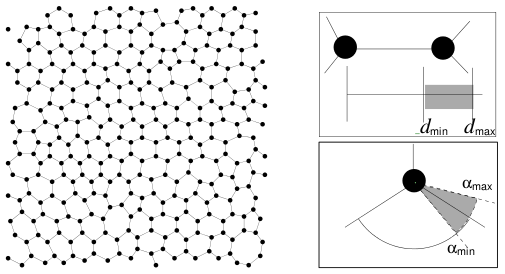
\includegraphics[width=0.4\textwidth]{Figures/amorphousSilicon.png}
	\caption{An example of an amorphous solid under simulation.  A maximum vertex number of 3 is defined, along with minimum and maximum angles and bond lengths; taken from: Ref. \protect\citenum{Peinado1997gwt}}
	\label{fig:amorphousSilicon}
\end{figure}


\section{Simulated Annealing}
Simulated annealing is a stochastic approach towards minimizing an energy function.

\section{Genetic Algorithms}
Genetic Algorithms are probabilistic search algorithms, which simulate natural evolution. They are based on the phenomenon of “survival of the fittest”. In nature, the fittest individuals are most likely to survive and mate, and their offspring are expected to be fitter and healthier.
The algorithm represents the search space of the problem, or the population as a collection of individual represented by character strings or chromosomes. The algorithm choses an initial randomly generated population, and determines the fitness of each individual in this population. The fitness of an individual is used to find the probability of crossover. Parents are chosen stochastically from this population, and are combined to produce children. From newly created individuals, a small number are chosen for mutation, i.e. their character string (genetic makeup) is changed at a randomly chosen mutation point. The individuals with least fitness are removed from the population after each iteration to reduce the population to its initial size. This new generation is then used in the next iteration and the process is repeated until a stopping criterion is reached, such as a maximum number of iteration or a specified fitness level. At this point the individual with maximum fitness is taken to be the optimal solution

\section{Ant-Colony Approaches}
Ant Colony Optimization~\cite{Dorigo96theant} draws inspiration from the behavior of ants as they develop a path from their nest to a food source.  As ants travel, they deposit pheromones.  These pheromones can be detected by other ants and the ants are more likely to follow a path with higher pheromone concentration.  In addition to the ants depositing pheromones, these pheromones will evaporate over time.  This means that shorter paths will allow larger pheromone concentrations to buildup as ants will be depositing pheromones quicker than they evaporate.  Eventually, the system will converge on a minimum solution.  A global minimum is pursued by starting out with a large number of ants and by tuning the weight at which pheromones influence decisions. 

\section{Go with the Winner Approaches}
Simulated annealing probabilistically convergences to the optimal solution at the rate
 of $O(\frac{1}{n})$ where n is the number of independent runs.  
Using heuristic schemes such as the ``Go with the Winner''~\cite{Aldous1994gwt}, hereby referred to as GWW, 
one can improve this convergence rate to $O(log \frac{1}{n})$ and have recently found their way into molecular modeling applications~\cite{Peinado1997gwt}.  In general terms, the GWW algorithm mirrors that of simulated annealing; however, each independent run is periodically reassessed to determine if one is converging upon a losing solution.  Runs with 
no chance for success are immediately discarded while runs with the best chance of finding an optimal solution
are replicated; thus, GWW generates an ensemble of independent runs filled with  ``winners''.  

\section{Analysis}
To test the scientific performance of these optimization schemes, we will study the convergence properties of minimization on particle reconstruction mapped onto the TSP.  Given that the deposition pattern of particles is not unique, all of the optimization schemes will need to generate an ensemble of possible models.
To quantify the phase space coverage of these optimization schemes, we will initially start from known particle configurations, such as a square and hexagonal lattices, generate multiple optimization trajectories, and will analyze the number and size of the clusters produced by each method to determine their overall  performance.  

Additionally, we will test the computational effort involved in each optimization scheme, focusing on the wall-clock time and number of alogrithm iterations/replicates are needed to sufficent converge to a reasonable answer.  If time permits, we will also test the ease of formulating these schemes into a parallel computing framework to improve their calculation efficiency.

\bibliographystyle{unsrt}
\bibliography{AtomicScaleProposal}
\end{document}
